\hyphenation{al-though Al-though}

\begin{abstract}

Today's tasks require a plethora of analytics tasks to be conducted to
tackle state-of-the-art computational challenges posed in society
impacting many areas including health care, automotive, banking,
natural language processing, image detection, and many more data analytics
related tasks. Sharing existing analytics functions allows reuse and reduces overall effort. However, integrating deployment frameworks in the age of cloud computing is often out of reach for domain experts. Simple frameworks are needed that allow even non-experts to deploy and host services in the cloud. To avoid vendor lock-in, we require a generalized composable analytics service framework that allows users to integrate their services and those offered in clouds, not only by one, but by many cloud compute and service providers.

We report on work that we conducted to provide a service integration framework for composing generalized analytics frameworks on multi-cloud providers that we call our Generalized AI Service (GAS) Generator. We demonstrate the framework's usability by showcasing useful analytics workflows on various cloud providers, including AWS, Azure, and Google and edge computing IoT devices. The examples are based on Scikit learn to use them also in educational settings that can easily be replicated and expanded upon. Benchmarks are used to compare the different services and showcase general replicability.

\end{abstract}


\maketitle

\tableofcontents

\verbatimfont{\footnotesize}%



\maketitle

\noindent\textbf{Keywords:} cloudmesh, AI service, REST, multi-cloud

\bigskip

\begin{footnotesize}
\smallskip\noindent
\textbf{Source Code:} \url{https://github.com/cloudmesh/cloudmesh-openapi}\\
\noindent \textbf{Status:} Draft version from \today.\\
\noindent \textbf{Link to newest version:} 
\Link{https://github.com/cloudmesh/cloudmesh-openapi/tree/main/paper}
\end{footnotesize}

\bigskip

\section{Introduction}


In today's application, scientists want to share their services with many colleagues while not only offering the services as bare metal programs but exposing the functionality as a Software as a Service (SaaS). This has the advantage that the services can be readily reused by other applications and hosted in the cloud, allowing access to state-of-the-art services or volumes of resources that otherwise would not be accessible to individual domain experts. Through the increased availability, resource constraints can be reduced, and scientists can offer their analytics workflows as services to the community. This may include long-lasting services envisioned by cloud computing as part of its Software as a Service (SaaS) paradigm or for smaller analytics functions as microservices. Furthermore, a subset of analytics functions can be offered as part of a serverless computing model, elevating the penetration from a pure bare metal solution to a multi-pronged cloud-based service offering.

While working with many professionals, researchers, and students, we found that the barriers to entry to accomplish this goal remain very high, and would elude many domain experts as they have neither the expertise nor the time to learn the expertise necessary to conduct the infrastructure-related tasks integrating DevOps and analytics tasks. Although recent developments, especially on the serverless computing side, have made progress, we ought to leverage the existing expertise of the domain scientists while automating the creation of various services from SaaS, microservices, and serverless computing.
Having worked with this community, we found that the educational steps involved for a beginner take about two to three months to get up to a level where the development of cloud-based services is possible. We set the goal to explore if it is possible to drastically reduce the time needed to create such services.

For this reason, we developed a sophisticated but easy to use framework that takes a regular python function and converts it automatically into a secure REST service and OpenAPI specifications \cite{openapi} that can be reused in the ecosystem of cloud services. We used this framework to create many AI-based REST services to showcase the approach's validity. We used examples from SciKit-learn \cite{scikit-learn} and benchmark the execution of the resulting REST services on various clouds and an IoT device. 

The paper is structured as follows. In \Section{sec:background} we will start with a very brief background section to allow domain experts to catch up with the terminology and concepts used in our architecture. The background analysis leads us to our requirements presented in \Section{sec:requirements} and our architectural design shown in \Section{sec:architecture}. Our benchmarks are collected in \Section{sec:benchmark}. We present our conclusion in \Section{sec:conclusion}.

In the appendix, a small number of useful notes are provided to ease replication of what we have achieved by others. In the final publication, the appendix can be removed with a link to our manual for the pilot framework presented here \cite{cloudmesh-manual, cloudmesh-openapi} where we will include the content of the appendix. 

\section{Background}
\label{sec:background}

In this background section, we provide a small summary of activities related to this research so that domain experts can get a small introduction to concepts that we use to implement our architecture. It is beyond the scope of this paper to give more detailed introductions in topics such as IaaS, SaaS, microservices, serverless computing, OpenAPI, and REST services. The sections will, however, be useful as a starting point for further research to the reader. 

\subsection{The Big Data Reference Architecture}

NIST has developed a Big Data Reference Architecture as part of the NIST Big Data Interoperability Framework (NBDIF)\cite{nist-v6} and identified several use cases that motivate
it \cite{nist-v3}. The reference architecture is depicted in \Figure{fig:bdra}. It includes the following components: Data Provider, Big Data Application Provider, Big Data Framework Provider, Data Consumer and
System Orchestrator as well as two overarching fabrics: security and
privacy and system management. There are three types of linkages,
namely \emph{Big Data Information flow}, \emph{Service Use and
  Software Tools}, and \emph{algorithms transfer}. The architecture
presents a level of abstraction to define Big Data
applications. Components that implement sophisticated functionality
work in concert to address the challenging creation of instantiating architectures beyond the conceptual stage. As such, the components
interact with each other that are expressed through the linkages
within the NBDIF.  The next logical step is to explore how it can
benefit and be used for analytics services.

\begin{figure}[htb]
\centering

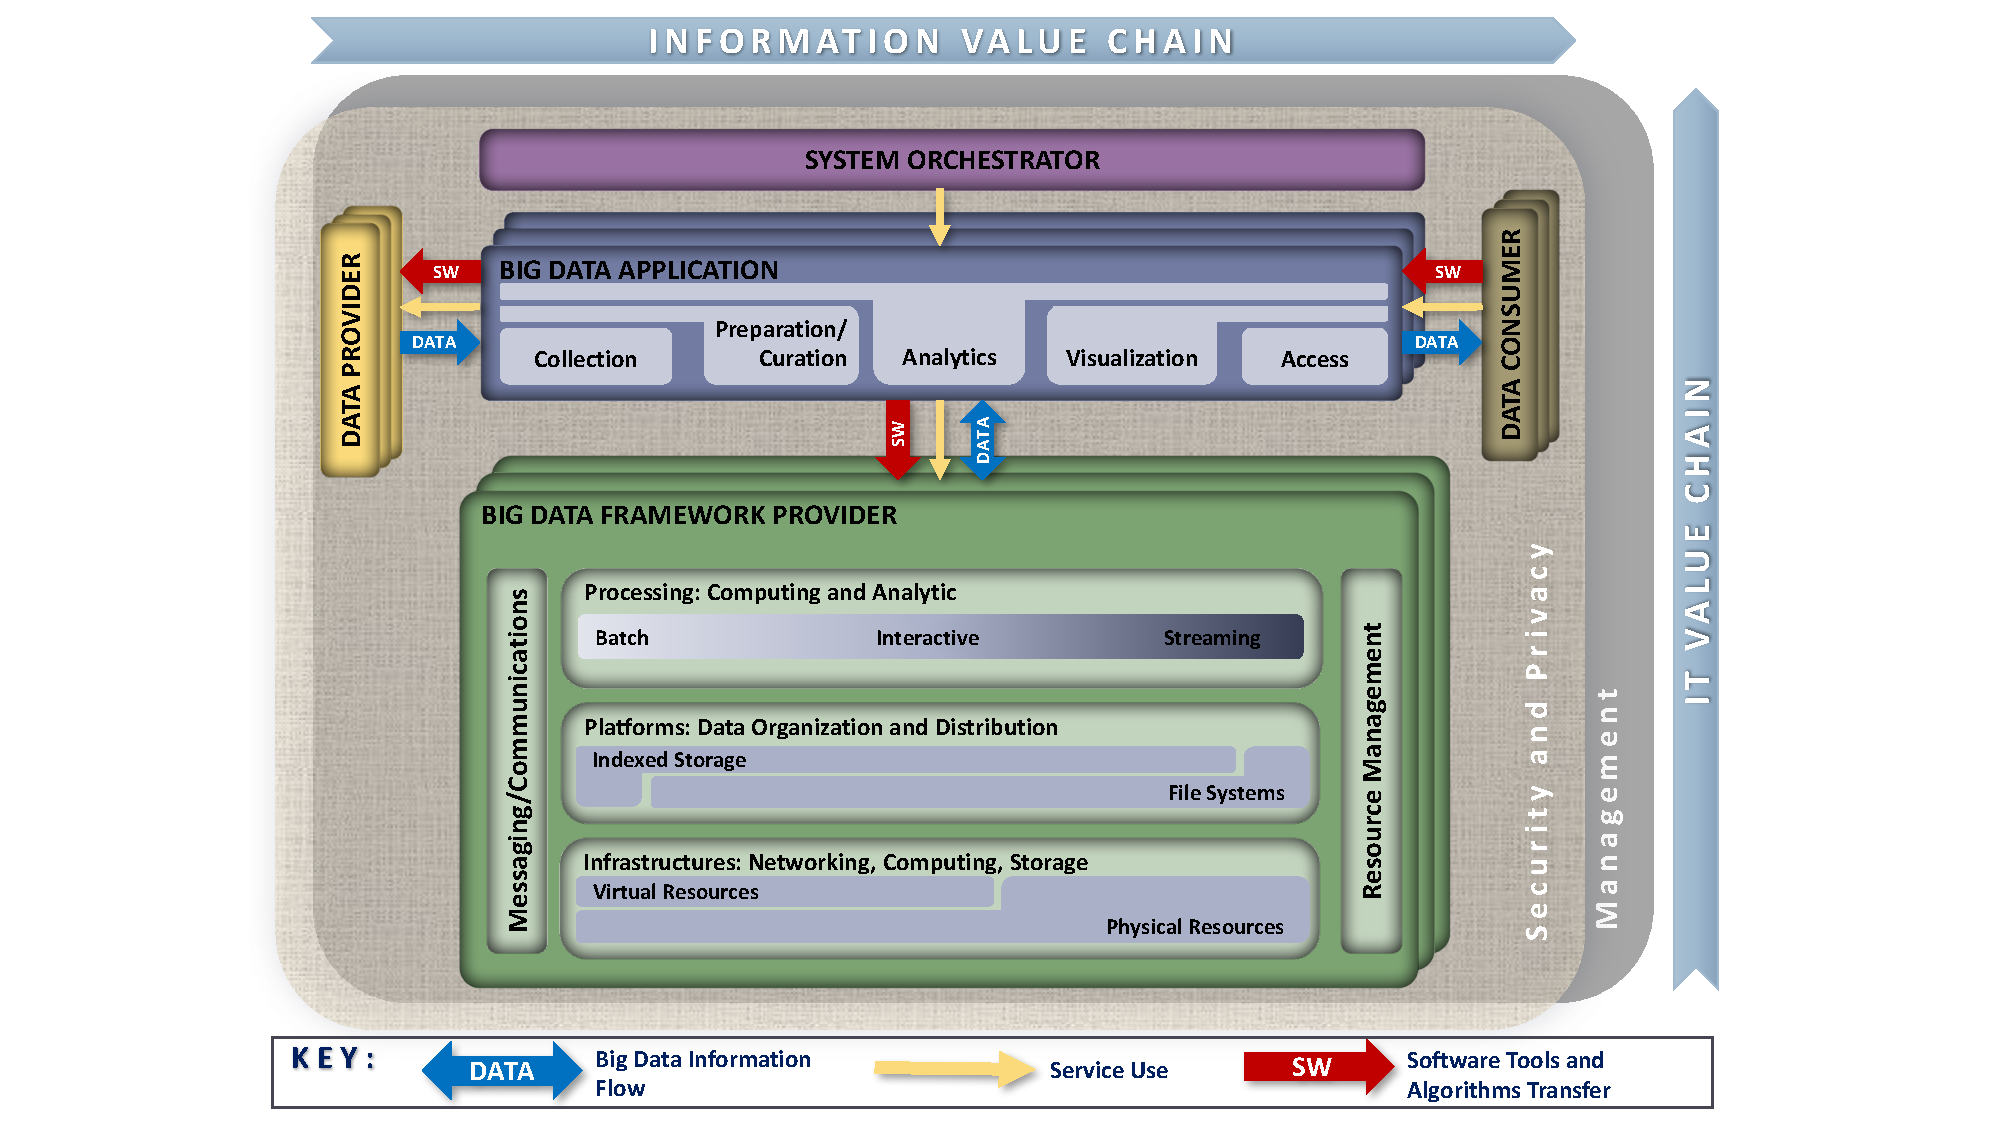
\includegraphics[width=1.0\columnwidth]{images/NIST_RA_latest-crop.pdf}

\caption{NIST Big Data Reference Architecture \cite{nist-v8}}

\label{fig:bdra}
\end{figure}

NIST has developed through open working group participation the
following documents related to the
NBDIF~\cite{nist-v1,nist-v2,nist-v3,nist-v4,nist-v5,nist-v6,nist-v7,nist-v8,nist-v9}. Within
these activities, Volume 8 is of especial importance as it allows a
set of Big Data Architectural needs
\cite{cloudmesh-openapi}\cite{las20book-cloudeng}. This effort builds the basis of
our activities reported here while expanding it to cloud providers and
services focusing on {\em Analytics Services}, which are not covered
by the current volumes. 

In a previous effort, we have developed a reference implementation that follows the architecture laid out in NBDIF and is easy to use by scientists. 
However, it focused mostly on multi-cloud provider access via REST services and command-line tools. The reference implementation is done as part of the cloudmesh project, which was one of the first hybrid multi-cloud provider interfaces, even including cloud technologies that are no longer active such as Eucalyptus \cite{www-eucalyptus}, OpenCirrus \cite{opencirrus}, FutureGrid \cite{futuregrid}, and Comet Cloud \cite{las-comet}. Today, it supports clouds such as AWS \cite{www-aws}, Azure \cite{www-azure}, Google Cloud Platform \cite{www-google}, Oracle \cite{www-oracle-cloud}, and OpenStack \cite{www-openStack}. It will offer further value as it also explores the integration of MapReduce frameworks such as Hadoop \cite{www-hadoop} and Spark \cite{www-spark}, as well as container-based frameworks such as Docker \cite{www-docker}, and Kubernetes \cite{www-kubernetes}. 

However, the work presented here focuses on creating analytics services that can be automatically created and hosted on any of the clouds supported by cloudmesh. This is a non-trivial effort due to the large number of technologies involved and is outside of the expertise of domain scientists. However, the use of cloudmesh makes it possible for the domain scientist to easily access these services and leverage our more than ten years of experience in this field.

The previous work provides us with a blueprint on how to proceed.  We list the following main findings of our earlier work that we leverage as part of this work.

\begin{description}
  
\item[Software Defined Analytics Services and Applications.] ~\\ 
  Just as
  in the NBDIF, the utilization of \emph{DevOps} to deliver
  Software-Defined (SD) Big Data applications is of
 utmost importance for the design of reusable services and components \cite{cloudmesh-manual,bigdata-stack-1,bigdata-stack-2}. 
  
\item[Multi-cloud Provider Interfaces.] Volume 8 was through community
  input shaped in such a form that it allows multi-cloud
  interfaces. Such interfaces have been in practical use in our software and showcase the validity of the NIST-BDRA approach. It is clear that we need to introduce such multi-cloud and multi-service
  interfaces for analytics-related tasks whenever possible as motivated in our introduction. 

\item[Use Case Collection.] NIST has provided as part of the NIST BDRA
  document Vol. 6~\cite{nist-v6} several use cases that can be analyzed and from which common big data services can be detected. These use
  cases were sufficient to drive the NIST BDRA document \cite{nist-v6}
  and allowed the community to investigate initial implementations. These use cases also motivate the work conducted in this effort.

\item[Independent API Specification Leveraging OpenAPI.] ~\\ Although the use of OpenAPI \cite{openapi,openapi-tools} is not required as part of the NIST specification, it can be used to formulate services in a
  language-independent fashion. Hence it allows {\em creating, evolving and promoting a vendor-neutral description format}. This is important to provide for our analytics services approach to promote a vendor-neutral and independent effort.

\item[API's and Tools Targeting A Multi-Layered Architecture.] In our
  previous effort, we learned that we need to provide support for
  tools, services, and APIs on multiple levels in a multi-layered
  architecture. While some users expect a generalized specification other users may require access on the command line, deployed services, or even a Jupyter notebook. We observe that in many cases,
  the entry-level to define API specification is too high for many. This is the case for domain experts in the analytics community that often lack the necessary expertise for general service integration and deployment.

\end{description}

Hence, previous work provides us with a blueprint on how to proceed, which we summarize as 
follows:

{\em Develop an easy to use framework that allows the scientists (a) to develop shareable analytics components (b) allow for the deployment of them, and (c) allow for the easy reuse of the services by community members leveraging the deployments.} 



\subsection{REST}\label{rest}

One of the most common architectural styles for cloud-related services is based on {\bf R}epr{\bf E}sentational {\bf S}tate {\bf T}ransfer (REST). REST often uses
the HTTP protocol for the CRUD functions, which create, read, update, and
delete resources. It is important to note that REST is not a standard,
but it is a software architectural style for building network services.
When referred to as a part of the HTTP protocol, REST has the methods of
GET, PUT, POST, and DELETE. These methods are used to implement the CRUD
functions on collections and items for which REST introduces abstractions for managing these collections and single resources \cite{las-book-cloud} as explained in \Figure{fig:rest}.


\begin{figure}[htb] 

\begin{adjustbox}{minipage=0.9\columnwidth,
                  margin=10pt 5pt,%
                  bgcolor={black!2},%
                  frame=0.01pt}%
{\footnotesize
\begin{description}
\item[Collection of resources.] Assume the URI,  \verb|http://.../resources/|, identifies a
  collection of resources. The following CRUD functions would be
  implemented:

  \begin{description}
  \item
    [GET:] List the URIs and details about the collection's
    items.
  \item[PUT:] Replace the collection with a different collection.
  \item[POST:] Make a new entry in the collection. The operation
    returns new entry's URI and assigns it automatically.
  \item
    [DELETE:] Delete the collection.
  \end{description}
  \bigskip

\item[Single Resource.] Assume the URI, \verb|http://.../resources/item1|, identifies a
  single resource in a collection. The following CRUD functions would be
  implemented:

  \begin{description}
  \item
    [GET:] Fetch a representation of the item in the collection,
    extracted in the appropriate media type.
  \item
    [PUT:] Replace the item in the collection. If the item does
    not exist, then create the item.
  \item
    [POST:] Typically, not used. Treat the item as a collection
    and make a new entry in it.
  \item
    [DELETE:] Delete the item in the collection.
  \end{description}
\end{description}
}
\end{adjustbox}
\caption{REST definitions for a collection and single resources.}
\label{fig:rest}
\end{figure}

Because REST has a defined structure, there are tools that manage
programming to REST style architectures. They include, for example, different categories
\cite{las-book-cloud}:

\begin{itemize}
\item \textbf{REST Specification Frameworks} which  define
  REST service specifications for generating REST services in a
  language and framework independent manner such as Swagger 2.0
  \cite{openapi-2}, OpenAPI 3.0 \cite{openapi-3} and RAML
  \cite{raml-1}.
\item \textbf{REST programming language support} which include tools and services
  for targeting specific programming languages such as Flask Restful
  \cite{www-flask-restful}, and Django Rest \cite{www-django-rest} for Python.
\item \textbf{REST documentation-based tools} which are tools to document
  REST specifications. One such tool is Swagger \cite{www-swagger}.
\item \textbf{REST design support tools} which support the
  design process in developing REST services while defining reusable client and server that can be integrated and enhanced such as Swagger \cite{www-swagger} and other tools
  available at OpenAPI Tools \cite{www-openapi-tools} to generate code
  from OpenAPI specifications \cite{www-swagger-codegen}
\end{itemize}

Within our work reported here, we will heavily base our architecture on REST. From this small discussion, it is evident that although the concept of REST is easy to understand, a significant amount of expertise is needed to apply it, which domain scientists may not be interested in to know but keen on reusing without needing to know the details.

\subsection{OpenAPI}

One of the important aspects of generating REST services is a language-independent formulation of REST services. For this reason, the ``OpenAPI Specification (OAS) defines a standard, language-agnostic interface to RESTful APIs which allows both humans and computers to discover and understand the capabilities of the service without access to source code, documentation, or through network traffic inspection. When properly defined, a consumer can understand and interact with the remote service with minimal implementation logic \cite{openapi}.''

Hence the specification allows us to not only display the documentation but also allows us to use it to generate the clients and server stubs from it automatically. OpenAPI can be formulated as a YAML Ain't Markup Language (YAML) \cite{www-yaml} file. 

An OpenAPI definition can then be used by documentation generation tools to display the API, code generation tools to generate servers and clients in various programming languages, testing tools, and many other use cases. One of the issues with using the OpenAPI during the design of a project is that it takes considerable effort to understand the specification. Based on our experience of integrating it into university courses, it is a formidable effort to learn and use it. The lessons from this educational effort that includes researchers, professionals, graduate, and undergraduate students motivated this work.

\subsection{Hybrid Multi-Cloud Computing with Cloudmesh}\label{cloudmesh}

Cloud computing providers offer their customers on-demand self-service
computing resources that are rapidly elastic and accessible via broad
network access \cite{nist-cloud-standard}.
They accomplish this through the economies of scale achieved by resource
pooling (serving multiple customers on the same hardware) and using
measured services for fine-grained customer billing \cite{nist-cloud-standard}.
Cloud providers offer these resources in multiple service models
including infrastructure as a service, platform as a service, software
as a service, and, recently, function as a service
\cite{nist-cloud-standard}.
These providers are rapidly offering new platforms and services ranging
from bare-metal machines to AI development platforms like Google's
TensorFlow Enterprise platform \cite{www-tensorflow-enterprise}, and AI services
such as Amazon's text-to-speech service \cite{amazon-polly}.

Customers can take advantage of cloud computing to reduce overhead
expenses, increase their speed and scale of service deployment, and
reduce development requirements by using cloud providers' platforms or
services. For example, customers' developing AI systems can utilize
clouds to handle big data inputs for which private infrastructure would
be too costly or slow to implement. However, having multiple competing
cloud providers leads to situations where service availability,
performance, and cost may vary. Customers must navigate these
heterogeneous solutions to meet their business needs while avoiding
vendor lock-in and managing organizational risk. This may require
comparing or using multiple cloud providers to meet various objectives.

Today's infrastructure deployments can benefit from a {\em hybrid multi-cloud}
strategy in which a mix of cloud-enabled services such as computing, storage, and other services 
are integrated from on-premises infrastructure, private cloud services, and a public cloud.

As pointed out earlier, Cloudmesh \cite{cloudmesh-manual} is a framework and toolkit that enables users to
easily access hybrid multi-cloud environments. Cloudmesh is an evolution of
previous tools that have been used by many users. Cloudmesh makes
interacting with clouds easy by creating a service mashup to access
common cloud services across numerous cloud platforms. Cloudmesh
contains a sophisticated command shell, a database to store JSON
objects representing virtual machines, storage, and a registry of REST
services \cite{cloudmesh-openapi}.  Cloudmesh has a sophisticated
plugin concept that is easy to use and leverages python namespaces
while integrating plugins from different source code
directories \cite{cloudmesh-github}.  Installation of Cloudmesh is
available for macOS, Linux, Windows, and Rasbian
\cite{cloudmesh-manual}.

Cloudmesh works with a variety of cloud providers, including Amazon Web
Services, Microsoft Azure, Google Cloud Platform, and Oracle's OpenStack
based providers such as the academic research serving Chameleon Cloud \cite{chameleon-cloud}.

Recently we have also explored containers and microservices. The work presented here summarizes some of this effort. With the help of a plugin {\em cloudmesh-openapi} We can generate REST services, including microservices and
containers, to organize its functions and code. In addition, cloudmesh can be distributed as a container and used in a containerized environment. Through this ability, cloudmesh services generated with {\em cloudmesh-openapi} can also be deployed on Kubernetes.


\section{Requirements}
\label{sec:requirements}

Next, we present the most critical requirements that motivated our architecture and design. We start with a set of general requirements.

\begin{description}

\item[Leveraging new Python features.] Python is a very popular choice with many data scientists. Our framework will leverage the newest Python 3 features such as {\em Typing Interface} \cite{www-python-typing} in order to increase robustness and future-proofing of our code base. 

\item[Ability to be used within Jupyter Notebooks.] ~\\
The framework must be able to integrate with Jupyter notebooks as they are very popular with today's data scientists. The functionality must be easily accessible not only as part of python programs but also within Jupyter notebooks. This is of special importance also for cloud services such as Google Colab \cite{google-colab} which for example, offers cloud-based Notebooks. 

\item[Easy of use] is a critical aspect of the framework that is to be addressed from the start by allowing for ease of creation, ease of deployment, and easy use of the generated services. This is accompanied by easy to use command-line tools.

\end{description}

Next, we list some more specific requirements that motivate our architectural design.

\begin{description}

\item[Multi-Cloud Service Integration.] The framework must allow us to integrate multiple cloud services, including IaaS, PaaS, and SaaS. This also includes the ability to access AI-based services offered by the various cloud providers.

\item[Hybrid-Cloud Service Integration.] The framework must allow integrating on-premise, private, and public clouds.


\item[Generalized Analytics Service Generator.] We need a generalized analytics service generator. The first step in the activity to generate an analytics service is to
provide an OpenAPI Service generator. Our generator will allow us to
define essential analytics functions such as (a) uploading and
downloading files to an analytics service; (b) specifying the
functionality through typing enhanced python functions; and (c)
generating the code for the service.

\item[Generalized Analytics Service Deployment.] After the service is generated, it needs to be deployed. For this step
we will be reusing the Cloudmesh deployment mechanism to instantiate
services on-demand on specified cloud providers such as AWS, Azure,
and Google. 

\item[Generalized Analytics Service Invocation.] The next step includes the invocation of the deployed services. While
analyzing some use cases, we identified that users often need to
invoke the same service many times to tune service parameters in a
quasi-realtime fashion while using parameters that can not be included in the URL. Hence we will need to upload input parameters through
files if the simple typing data types provided by our proposed
framework is not sufficient. 

\item[REST Services Architecture.] As REST has become the most prominent architectural design principle, our Generalized service architecture needs to be able to produce REST services.

\item[Automated REST Service Generation for other Languages.] Our framework must have provisions included that allow the integration into other programming languages and, on the other hand, allows the integration of services and functions developed in other languages.


  
\item[Generalized Analytics Service Registry.] As users and communities may develop many different services, we must provide the ability to  (a) find
specifications of generalized analytics services (b) find use-cases
of generalized analytics services (c) find infrastructure on which
such services can be deployed, and (d) find deployed analytics
services. For this, we need a registry that can be queried by the community.

\item[Generalized Composable Analytics Services.] Services must be allowed to reuse other services to allow for easy integration. Thus we need to make our services composable. This also includes the choreography of the execution of such composable services.




\end{description}


\section{Architecture}
\label{sec:architecture}

To satisfy our requirements, we have designed a multilayered architecture delivering a framework and toolkit to allow the easy generation and deployment of generalized AI-based REST services. 

It contains two main layers. The first layer is concerned with generating the REST services, while the second focuses on easy deployment in a multi-cloud environment. However, as we also deal with hybrid infrastructure, we allow in the second layer access to HPC and local on premise resources. In addition, our architecture addresses the creation of containers and their deployment in docker and Kubernetes. This way our framework is not only capable of delopying into cloud virtual machines, but also into other infrastructure services, either offered locally or in the cloud. Both layers can be accessed and control via a convenient Command shell and client. As they are REST services, the deployed services can easily be accessed from other resources via the REST API. Next, we describe some of the important features within each of the layers while starting with the infrastructure deployment. 

\subsection{IaaS Access Layer}

This layer allows us to deploy different infrastructure services on demand while introducing an abstraction layer for compute resources that allow IaaS access across the different platform offerings. Here, we can leverage from the cloudmesh toolkit that provides us with the basic interfaces to virtual machines to conveniently access in homogeneous fashion AWS, Azure, Google, Oracle, and OpenStack. Access to HPC and Bare metal can be integrated and has been showcased in the past in cloudmesh. We also have prototyped in cloudmesh interfaces for accessing compute resources via docker and Kubernetes. 

All of the deployment can easily be managed through a simple client shell that can also be used as a command line executor. This system is one of the key components of cloudmesh and allows easy integration of new commands and modules. This makes cloudmesh extensible, while others can provide new functionality that can be accessed in the command shell and command line interpreter. We use the cloudmesh command shell to integrate the functionality of the Generalized AI Service (GAS) Generator and describe its functionality in more detail next.

\subsection{GAS Generator}

The Generalized AI Service (GAS)\footnote{{\em GAS} the name GAS is derived from two different common usages. First, it refers to gasoline, referring to fuel that we need to generate the services; the second is an expandable material that fills the whole of a container. If you have better ideas or analogies for naming our framework, please get in contact with us. We love to hear from you!} Generator creates the REST service from a simple function or class definition while utilizing the newest python language features such as documented typing information integrated in the program specification. The GAS Generator provides us with the {\em fuel} that is needed as part of the service deployment. This is manifested in a number of artifacts for the deployment. The artifacts include a specification derived from the python program in OpenAPI format, the server code that is derived from the OpenAPI format, and an optional container specification file (e.g., Dockerfile). In addition, as we expect that the service is going to be reused, we use a GAS Service registry in which we record the specification description of the service as well as deployment information on which the service ought to be deployed. This deployment specification can be derived from other prototype cloudmesh components such as cloudmesh-frugal, which can obtain resources based on minimal cost. We have not explicitly included this component in our architecture picture as we have not used it as part of our benchmarks that we describe later. 

% \TODO{mod image to add a backlink to the user}

\OneFIGURE
    {openapi-arch-new-2.pdf}
    {Layered architecture of the cloudmesh OpenAPI framework.}
    {fig:arch-new}

\subsection{GAS Workflow}

To showcase why the framework is so useful for data scientists, we are contrasting the definition workflow that a scientist undergoes while using OpenAPI without and with GAS Generator in  \Figure{fig:flow-schema} and \Figure{fig:flow-function}.

The workflow in  \Figure{fig:flow-schema} showcases a typical workflow as promoted by the developers of Swagger codegen \cite{www-swagger-codegen}. The user identifies from his use case an OpenAPI schema that is used to generate the code. However, this is an unnecessary high entry barrier as the creation of these schemas is complex. While using the swagger code generator, a variety of code stubs in many different languages can be created. The code generated requires an unnecessary high entry barrier as we next need to identify how and where we include an implementation of a function that we want to expose as a REST service. Once complete, the rest of the activity requires the remaining steps to be executed by hand, but scripts could be developed to automatize it. 

Next, we like to contrast this with our much-simplified approach. As we know, the data scientists have the knowledge to write python function (or class); we simply leverage this expertise and take the function (or class) and provide it as input (fuel) to the GAS generator. This is done with a simple one-line command invocation that just includes the name of the python program in which the function (or class) is defined. The scientist does not have to learn REST, the scientist does not have to look into a code stub that is generated for him, the scientist doe not even have to know how to instantiate or run the service. Furthermore, the scientist does not have to know about any security as we have added features to the code to leverage the existing security mechanism as a simple flag to the GAS Generator command line instantiation. This simplification allows the scientist to develop REST services in minutes rather than a month as the entry barrier is very low. Additionally, as we are integrated with cloudmesh infrastructure deployments, the instantiation of the services can also be done with a one line command under the assumption the scientist has accounts registered with cloudmesh allowing him to authenticate and authorize the deployment of the services in the cloud. 

\begin{figure}[htb]

\begin{minipage}[b]{0.48\columnwidth}
\begin{center}
\begin{adjustbox}{width=1.0\columnwidth}
\begin{footnotesize}
\forestset{
  skan tree/.style={
    for tree={
      drop shadow,
      text width=3cm,
      %grow'=0,
      %growth=south,
      rounded corners,
      draw,
      top color=white,
      bottom color=blue!20,
      edge={Latex-},
      child anchor=parent,
      %parent anchor=children,
      anchor=parent,
      tier/.wrap pgfmath arg={tier ##1}{level()},
      s sep+=2.5pt,
      l sep+=2.5pt,
      edge path'={
        (.child anchor) -- (!u.parent anchor)
      },
      node options={ align=center },
    },
    before typesetting nodes={
      for tree={
        content/.wrap value={\strut ##1},
      },
    },
  },
}
\begin{forest}
  skan tree
  [Usecase, \nwhite
    [Schema, \nwhite
       [Code Generator (31 Languages), \ngreen
          [Implementation, \nwhite
          [Function, \nwhite
          [Service, \ngreen
             [Deployment, \nred
               [Verification, \nred
                  [Hosting, \nred
                  ]
               ]
               ]
            ]
            ]
         ]
      ]
    ]
  ]
\end{forest}
\end{footnotesize}
\end{adjustbox}
\end{center}
%\vspace{-0.8cm}
\caption{Schema-based component flow to specify an analytics service.}
\label{fig:flow-schema}

\end{minipage}
\ \
\begin{minipage}[b]{0.48\columnwidth}
\begin{center}
\begin{adjustbox}{width=1.0\columnwidth}
\begin{footnotesize}
\forestset{
  skan tree/.style={
    for tree={
      drop shadow,
      text width=3cm,
      %grow'=0,
      %growth=south,
      rounded corners,
      draw,
      top color=white,
      bottom color=blue!20,
      edge={Latex-},
      child anchor=parent,
      %parent anchor=children,
      anchor=parent,
      tier/.wrap pgfmath arg={tier ##1}{level()},
      s sep+=2.5pt,
      l sep+=2.5pt,
      edge path'={
        (.child anchor) -- (!u.parent anchor)
      },
      node options={ align=center },
    },
    before typesetting nodes={
      for tree={
        content/.wrap value={\strut ##1},
      },
    },
  },
}
\begin{forest}
  skan tree
  [Usecase, \nwhite
  [Function, \nwhite
    [Schema Generator, \ngreen
       [Schema, \ngreen
           [Service, \ngreen
             [Deployment, \nred
               [Verification, \nred
                  [Hosting, \nred
                  ]
               ]
            ]
        ]
      ]
    ]
    ]
  ]
\end{forest}
\end{footnotesize}
\end{adjustbox}
\end{center}
%\vspace{-0.8cm}
\caption{Function-based component flow to specify an analytics service.}
\label{fig:flow-function}

\end{minipage}

\end{figure}


\subsection{Scripting as Fuel for the GAS Generator}

Next, we demonstrate through two examples of how simple it is to obtain Services from python specifications. In our example, we define one that uses a function definition returning a result. We chose a simple add function and list the code related to it in \Figure{fig:function}. We also expand upon the example and use a class definition to showcase how to derive services using multiple paths instead of being deployed in different services as showcased in \Figure{fig:class}. As we see from the example, other than using the new typing feature provided in Python, the example is just a regular Python program. It can be tested locally on the system to check its functionality before we generate the service.

\Figure{fig:deploy-function} shows how to generate and deploy the service. As this process is the same for the class-based definition and only differs in the filename, we omitted it to include an explicit listing of the access method for it.

Once the service is deployed the {\em curl} calls in \Figure{fig:function-curl} and \Figure{fig:class-curl} showcase how to interact with the service from the command line. Naturally, one can use any programming language that has built-in libraries for HTTP requests to interface with the service (such as {\em requests} in Python \cite{www-python-requests}). 
Once we execute the following lines in a terminal, the result of the
the addition will be calculated in the REST service, and it is returned.

\newcommand{\FONT}{\tiny}


\begin{figure}[htb]
\begin{lstlisting}[language=Python,
                   basicstyle=\ttfamily\FONT,
                   numbers=left,                   
                   numbersep=5pt,
                   xleftmargin=5mm]
def add(x: float, y: float) -> float:
    """
    adding x and y.
    :param x: x value
    :param y: y value
    :return: result
    """
    result = x + y
    return result
\end{lstlisting}
\caption{Defining an analytics function that is used to generate a REST service.}
\label{fig:function}
\bigskip
\begin{lstlisting}[language=bash,
                   firstnumber=10,
                   basicstyle=\ttfamily\tiny,
                   numbers=left,                   
                   numbersep=5pt,
                   xleftmargin=5mm]
$ cms openapi generate add --filename=./add.py
$ cms openapi server start ./add.yaml 
$ curl \ 
 -X GET "http://localhost:8080/cloudmesh/add?x=1&y=2" -H "accept: text/plain"
# This command returns
> 3.0
\end{lstlisting}
\caption{Generating, deploying, and invoking the REST service. {\color{white}aaaaaaaa}}
\label{fig:deploy-function}
\label{fig:function-curl}
\bigskip
\begin{lstlisting}[language=Python,
                   basicstyle=\ttfamily\FONT,
                   numbers=left,                   
                   numbersep=5pt,
                   xleftmargin=5mm]
class Calculator:

    @classmethod
    def multiply(cls, x: int, y: int) -> int:
        """
        Multiply int by int and return an int.

        :param x: the value of input #1
        :param y: the value of input #2
        :return: result of multiplying x by y
        """
        return x * y

    @classmethod
    def divide(cls, x: int, y: float) -> float:
        """
        Divide int by float and return a float.

        :param x: the value of input #1
        :param y: the value of input #2
        :return: result of dividing x by y
        """
        return x / y

if __name__ == '__main__':
    calc = Calculator()
    print("multiply 1 * 2: ",  calc.multiply(1, 2))
    print("divide 6 / 3.14: ",  calc.divide(6, 2.3))

\end{lstlisting}

\caption{Defining an analytics function with the help of class methods to generate a REST service with multiple functions.}
\label{fig:class}

\bigskip
\begin{lstlisting}[language=Python,
                   firstnumber=29,
                   basicstyle=\ttfamily\FONT,
                   numbers=left,                   
                   numbersep=5pt,
                   xleftmargin=5mm]
$ curl \ 
  -X GET "http://localhost:8080/cloudmesh/multiply?x=1&y=2" \
  -H "accept: text/plain"

$ curl \ 
  -X GET "http://localhost:8080/cloudmesh/divide?x=6&y=3.14" \
  -H "accept: text/plain"

\end{lstlisting}

\caption{Defining an analytics function with the help of class methods to generate a REST service with multiple functions.}
\label{fig:class-curl}

\end{figure}


\subsection{GAS Security}

As we leverage OpenAPI and automatically generated OpenAPI services, it is possible to leverage security mechanisms from the underlying service implementation. To showcase this ability, we added basic authentication into our framework as an example configuration. However, it is certainly possible to extend this as the services we use also support OAuth, ApiKey Authentication, Bearer Authentication (JWT), and HTTPS support \cite{connexion-security}\cite{cloudmesh-openapi}.

To demonstrate basic authentication, a cloudmesh user can create an OpenAPI server whose endpoints are only
accessible as an authorized user. Currently, when basic auth is used, all endpoints are secured with this method. In future versions, we intend to allow securing selected methods.
An example of the usage of basic auth is provided on our Web page at \cite{www-cloudmesh-openapi-security}.

\section{Deployment Scenarios}

Due to the versatility of REST and our ability to integrate with a variety of infrastructure services, a rich set of deployment scenarios is possible. Two important scenarios related to single and multiple service provider deployments are discussed next. 

\subsection{Single Cloud Provider Hosted AI Service}

In this scenario, a user deploys Cloudmesh OpenAPI on a virtual machine from a cloud provider and uses it to host auto-generated, RESTful, AI services. Next, the scientist constructs an AI service as a set of Python functions that implement a workflow, for example, downloading data from a remote server, training an AI model, uploading a new sample for prediction, and running a prediction on that sample. After the deployment, the service is accessible using
standard HTTP request methods. In \Figure{fig:1} we show a remote client
that accesses such a typical AI service workflow.
Here the service is just deployed on a virtual
machine from a single cloud provider. Cloudmesh provides the
choice on which infrastructure provider to place the service. Through our security mechanism, the service can either be exposed to the public or to authenticated and authorized users.

\OneFIGURE
  {architecture-openapi-1.pdf}
  {Example AI Service Workflow to obtain data, train, upload data for prediction, as well as the interaction with it.}
  {fig:1}

\subsection{Multi-Cloud Hosted AI Service}

In our next scenario, we like to depict that it is possible to deploy the same service on multiple clouds through the use of our sophisticated but easy to use command clients. Detailed information about the exact commands are provided in our manual \cite{cloudmesh-manual}. Through this we can, for example, evaluate suitable providers for our deployment through benchmarking the service execution on each provider. This is precisely what we will be showcasing in our benchmark section and demonstrate this approach's feasibility. Thus the scientist not only obtains the ability with GAS Generator to develop and deploy services, but also to evaluate their performance on a variety of infrastructures. An example is provided in \Figure{fig:2} where a scientist deploys, for example, a service on AWS, Azure, and Google. As they are asynchronous services, the scientist can query the services simultaneously and
gathers responses and benchmarks. Obviously, this can be used in a real scenario to  integrate compute resources from multiple providers that can be accessed via our GAS services. It also allows specific adaptations such as the integration of cloud AI services with one provider that are not accessible in another. Hence the framework can also be utilized to benchmark secondary services that are offered by a particular provider, or if they are offered by more than one, they can be comparatively evaluated. 


\OneFIGURE
  {architecture-openapi-2.pdf}
  {Mult-Cloud AI Services: A client simultaneously accesses an AI service hosted
   on three separate cloud providers, AWS, Azure, and Google, to benchmark
   provider performance.}
  {fig:2}
 



\section{Benchmark}
\label{sec:benchmark}

In this section we describe our benchmark results.

\subsection{Infrastructure}

For a comparison of our services, we want to compare service deployments on virtual machines that are hosted on various cloud providers. We have chosen to select similar virtual machines for conducting the benchmark. This includes AWS \cite{www-aws}, Azure\cite{www-azure}, and Google \cite{www-google}. 

In addition, we are performing some bare metal experiments on two Raspberry PI clusters, one with Raspberry PI4's and the other with Raspberry PI 3b+'s. The latter has a management node, a PI 4, and worker nodes that are PI 3b+. The inclusion of the Raspberry platform was important to us as it demonstrates the capability of IoT and Edge computing devices that may become more prevalent in the future for delegating tasks to the edge. We further provide a docker container for a comparison of containerized services.


\subsection{Application}

We developed benchmark tests that are pytest replications of Scikit-learn artificial intelligent algorithms. These pytests are then run on different cloud services to benchmark statistics on how they perform. 

The team obtained cloud service
accounts from AWS, Azure, Google, and OpenStack. To deploy the pytests,
the team used Cloudmesh and its OpenAPI based REST services to
benchmark the performance on different cloud services. 

Benchmarks include components like data transfer time, model train time, model prediction time, and more. Besides this report, scripts and other code are provided for others to replicate our tests.

We provide two example benchmarks for the Eigenfaces SVM example. The
first deploys and measures the AI service on a single cloud provider at
a time (see \ref{single-cloud-provider-service-benchmarking}), and the second deploys a multi-cloud (see \ref{sec-multi-benchmark}) AI service measuring the service across the clouds in parallel.


\subsection{Algorithms and Datasets}
\label{sec:algorithms-and-datasets}

This project uses a simple example algorithm and dataset. We have chosen to use an example included in Scikit-learn as they are
widely known and can be used by others to replicate our benchmarks
easily. Nevertheless, it will be possible to easily integrate other data
sources, as well as algorithms, due to the generative nature of our code base for creating REST services. Within Scikit-learn we have chosen the {\bf\em Eigenfaces SVM Facial Recognition} example as it represents a very common data science usage pattern. This example conducts a facial recognition
that first utilizes principle component analysis (PCA) to
generate eigenfaces from the training image data, and then trains and
tests an SVM model \cite{www-skikit-learn-faces}. This example uses the real world {\em Labeled Faces in the Wild} dataset
consisting of labeled images of famous individuals gathered from the
internet \cite{faces-data}.


%  \textbf{Pipelined ANOVA SVM}: An example code that shows a pipeline
%  successively running a univariate feature selection with anova and
%  then a SVM of the selected features \cite{www-skikit-learn-pipeline}


\subsection{VM Selection}\label{vm-selection}

When benchmarking cloud performance, it is important to identify and
control VM deployment parameters. This allows one to analyze comparable service offerings, or identify
opportunities for performance improvement by varying deployment features
such as machine size, location, network, or storage hardware. These
benchmark examples aimed to create similar machines across all three clouds, and
measure their service performance. See \Table{tab:iaas} for a summary of the parameters
controlled in these benchmark examples.

One key component is the virtual machine size, which determines the
number of vCPUs, the amount of memory, attached storage types, and
resource sharing policies. Resource sharing policies include shared
core machine varieties—which providers offer at less expensive rates—that allow the virtual machines to burst over its base clock rate in
exchange for credits or the machine's inherent bursting factor
\cite{amazon-instances,google-instances}. For this example, we chose
three similar machine sizes that had comparable: vCPUs, underlying processors, memory, price, and were not a shared core variety. We installed the same Ubuntu 20.04 operating system on all
three clouds.

Another factor that can affect performance, particularly in network
latency, is the zone and region selected. We deploy all benchmark
machines to zones on the east coast of the United States. This helps
control variations caused by network routing latency and provides more
insight into the inherent network performance of the individual cloud
services.

%\rowcolors{2}{gray!25}{white}

Because cloud providers can observe varying loads during the day, the benchmark execution time is another parameter to control. In our single cloud provider benchmark for the Eigenfaces SVM example, clouds were tested at least twice and were run sequentially between the hours of approximately 19:45 EST and 03:30 EST starting with Google and ending with Azure. In the Eigenfaces SVM example, only 60 runs were
conducted on Azure due to a failed VM deployment caused by factors outside of the benchmark script's control. Compared to our single cloud provider benchmark, our multi-cloud benchmark benefits from all clouds being tested at the same time.

\begin{table}
  
\caption{Controlled VM parameters for cloud benchmarks.}
\label{tab:iaas}

\resizebox{1.0\columnwidth}{!}{
\begin{tabular}[]{@{}llll@{}}
\toprule
 & AWS & Azure & Google \tabularnewline
\midrule
%\endhead
Size (flavor) & m4.large & Standard\_D2s\_v3 & n1-standard-2 \tabularnewline
vCPU & 2 & 2 & 2 \tabularnewline
Memory (GB) & 8 & 8 & 7.5 \tabularnewline
Image & ami-0dba2cb6798deb6d8
& \begin{minipage}[t]{0.40\columnwidth}\raggedright
Canonical:0001-com-ubuntu-server-focal:20\_04-lts:20.04.202006100\strut
\end{minipage} & 
ubuntu-2004-lts
\tabularnewline
OS & Ubuntu 20.04 LTS & Ubuntu 20.04 LTS & Ubuntu 20.04 LTS \tabularnewline
Region & us-east-1 & eastus & us-east1 \tabularnewline
Zone &  N/A &  N/A & us-east1-b \tabularnewline
Price (\$/hr) &  0.1 & 0.096 & 0.0949995 \tabularnewline
%Runs/Test & 90 & 60 & 90\tabularnewline
\bottomrule
\end{tabular}
}
\bigskip

\caption{Raspberry Pi and Docker Specifications}
\label{tab:pi}
\resizebox{1.0\columnwidth}{!}{
\begin{tabular}[]{lllll}
\toprule 
&        &      &  Docker     & MacBook \tabularnewline
& Pi 3B+ & Pi 4 & (On MBP) & Pro i5 3.1GHz\tabularnewline
\midrule
%\endhead
Cores & 4 & 4 & 2&2\tabularnewline
Memory (GB) & 1 & 8  & 2&8\tabularnewline
OS & Raspberry OS 10 & Raspberry OS 10 & Ubuntu 20.04 LTS & macOS \tabularnewline
Version & Kernel 5.4.51  & Kernel 5.4.51 & NA& Big Sur \tabularnewline
Purchase Cost (\$) & 51.99 & 109.99 & NA& NA\tabularnewline
Energy Cost (\$/year) & 5.36 & 6.73 & NA & NA\tabularnewline
Price (\$/hr) &  0.0065 & 0.0133 & NA & NA\tabularnewline
%Runs/Test & 30 &  30 & 1 &\tabularnewline
\bottomrule
\end{tabular}
}


\smallskip 
{\footnotesize 
The Price is the purchase cost and 1yr energy cost, amortized over a year and given for each hour of the year.}
\end{table}

\subsection{Single Cloud Provider AI Service Benchmark.}
\label{single-cloud-provider-service-benchmarking}

The benchmark script for the Eigenfaces SVM example uses Cloudmesh to
create virtual machines and set up a Cloudmesh OpenAPI environment
sequentially across the three measured clouds, Amazon, Azure,
and Google. After the script sets up the environment, it runs a series
of pytests that generate and launch the Eigenfaces-SVM OpenAPI service,
and then conducts runtime measurements of various service functions. Also, we run the same pytests on two Raspberry Pi models, a MacBook Pro running a Docker container, and a bare metal MacBook Pro to demonstrate Cloudmesh OpenAPI's flexibility for multi-platform use.

The benchmark runs the pytest in two configurations. After the benchmark
the script sets up a virtual machine environment, it runs the first pytest
locally on the OpenAPI server and measures five runtimes:

\begin{enumerate}
\def\labelenumi{\arabic{enumi}.}
\item \textbf{download data:} Download and extraction of remote image data from
  ndownloader.figshare.com/files/5976015
\item \textbf{train:} 
  The model training time when run as an OpenAPI service
\item \textbf{scikitlearn train:} 
  The model training time when run as the Scikit-learn example without
  OpenAPI involvement
\item \textbf{upload local:} 
  The time to upload an image from the server to itself
\item \textbf{predict local:} 
  The time to predict and return the target label of the uploaded image
\end{enumerate}

The benchmark runs the second pytest iteration as a remote client and interacts with the deployed OpenAPI service over the internet. It tests two runtimes:

\begin{enumerate}
\def\labelenumi{\arabic{enumi}.}
\item \textbf{upload remote:} 
  The time to upload an image to the remote OpenAPI server
\item \textbf{predict remote:} 
  The time to run the predict function on the remote OpenAPI server, and
  return the target label of the uploaded image
\end{enumerate}

In \Figure{fig:download} we compare the download and extraction time of the labeled faces in the wild data set. This data set is approximately 233 MBs
compressed, which allows us to measure a non-trivial data transfer.
Lower transfer times imply the cloud has higher throughput from the data
server, less latency to the data server, or that the cloud has a better performing internal network. The standard deviation is displayed to compare the variation in the download times. Because the difference between commercial and residential internet speeds dominates the function runtime, we do not compare the clouds to the Pi models, MacBook, or docker container.
\begin{comment}
In  \Figure{fig:download} we show the same plot without the Pi and docker results to allow a closer comparison of the three comparable clouds.
\end{comment}

\begin{comment}
\TwoFIGURES
    {sample_graph_1_pi1.pdf}
    {Runtime for downloading the data used in the Eigenfaces SVM benchmark.}
    {fig:download_pi}
    {sample_graph_1.pdf}
    {Closeup of the Runtime for downloading the data used in the Eigenfaces SVM benchmark while excluding the runtime for the Raspberry PI.}
    {fig:download}
\end{comment}

\OneFIGURE
    {sample_graph_1.pdf}
    {Runtime for downloading the data used in the Eigenfaces SVM benchmark.}
    {fig:download}
    
In \Figure{fig:train_pi} we measure the training time of the Eigenfaces-SVM model both as an OpenAPI service and as the basic Scikit-learn example. This
allows us to measure the runtime overhead added by OpenAPI compared to the
source example. Here, the two functions are identical except that the
OpenAPI train function makes an additional function call to store the
model to disk. This is necessary to share the model across
the train and predict functions. In the figure there are two bars per cloud provider. The blue bars are the training time of the model when hosted as a Cloudmesh OpenAPI function. The
orange bars are the training time of the Scikit-learn example code without Cloudmesh OpenAPI involvement. The bars plot the mean runtimes and the error bar reflects the standard deviation of the runtimes. In  \Figure{fig:train} we show the same plot without the Pi models, MacBook, and docker results to allow a closer comparison of the three comparable clouds.

\TwoFIGURES
    {sample_graph_2_pi1.pdf}
    {Runtime for training on the data used in the Eigenfaces SVM benchmark.}
    {fig:train_pi}
    {sample_graph_2.pdf}
    {Closeup of the Runtime for training on  the data used in the Eigenfaces SVM benchmark without the data for the Pi.}
    {fig:train}


In \Figure{fig:upload_pi} we measure the time to upload an image to the server both
from itself and from a remote client. This allows us to compare the
function runtime as experienced by the server, and as experienced by a
remote client. The difference helps determine the network latency
between the benchmark client and the cloud service. In the figure, there are two bars per
cloud provider. The blue bars are the runtime of the upload function as
experienced by the server, and the orange as experienced by the remote
client. The bars plot the mean runtimes and the error bar reflects the
standard deviation of the runtimes. For the Pi models, MacBook, and docker container, we only measure the local function runtime.

%\TwoFIGURES
\OneFIGURE
    {sample_graph_3_pi1.pdf}
    {Runtime for uploading the data used in the Eigenfaces SVM benchmark.}
    {fig:upload_pi}
    %{sample_graph_3.pdf}
    %{Closeup of the Runtime for uploading the data used in the Eigenfaces SVM benchmark without the data for the Pi.}
    %{fig:upload}

In \Figure{fig:predict_pi} we measure the time to call the predict function on the uploaded image. Again we run this once from the local server itself, and a second time from a remote client to determine client and server runtimes. In the figure, there are two bars per cloud provider. The blue bars are the run time of the predict function as experienced by the server, and the orange as experienced by the remote client. The bars plot mean runtimes and the error bar reflects the standard deviation of the runtimes. For the Pi models, MacBook, and docker container, we only measured the local function runtime.

%\TwoFIGURES
\OneFIGURE
    {sample_graph_4_pi1.pdf}
    {Runtime for the prediction used in the Eigenfaces SVM benchmark.}
    {fig:predict_pi}
    %{sample_graph_4.pdf}
    %{Closeup of the Runtime for the prediction used in the Eigenfaces SVM benchmark without the data for the Pi.}
    %{fig:predict}

\Table{tab:2} presents a full listing of test results. For the upload and predict tests, the 'type' column denotes whether the test was run locally (server runtime) or remote (client runtime).

In \Table{tab:cost} we present a cost analysis of the service functions. The analysis uses the price from \Table{tab:iaas} and \Table{tab:pi}. The price for the cloud virtual machines are based on provider advertised costs, while the price for the Pi models are based on the hardware cost and one year of energy cost amortized for one year. This does not include other costs such as cooling, networking, or real estate. For the Pi energy cost we assume a full and constant load. We utilize power consumption benchmarks from \cite{pi-power} and Indiana residential kWH cost from \cite{indiana-energy} to calculate the expected Energy Cost per year. We calculate the cost to run each function and compare the clouds and Raspberry Pi 4 to the Raspberry Pi 3b+. We compare the percent runtime decrease from the Pi 3b+ to the clouds and Raspberry Pi4, and the percent cost increase from the Pi 3b+ to the clouds and Raspberry Pi 4.

\begin{comment}

\begin{table}[h]
%\caption{example table with vertical labels}
example for vertical labels
\centering
\begin{tabular}{clllrrrr}
\toprule
type & \multicolumn{1}{c}{test} & \multicolumn{1}{c}{cloud} & \multicolumn{1}{c}{mean} & \multicolumn{1}{c}{min} & \multicolumn{1}{c}{max} & \multicolumn{1}{c}{std}\\ 
\hline
\multirow{3}{*}{\rotatebox[origin=c]{90}{\parbox[c]{1cm}{\centering local}}} & 
\multirow{3}{*}{\rotatebox[origin=c]{90}{\parbox[c]{1cm}{\centering down\-load}}} 
  & aws &2&3&4&5\\
& & azure & 2&3&4&5\\
& & google &3&3&4&5\\ 
\hline
\multirow{3}{*}{\rotatebox[origin=c]{90}{\parbox[c]{1cm}{\centering local}}} & 
\multirow{3}{*}{\rotatebox[origin=c]{90}{\parbox[c]{1cm}{\centering predict}}} 
  & aws &2&3&4&5\\
& & azure & 2&3&4&5\\
& & google &3&3&4&5\\ 
\hline
\multirow{3}{*}{\rotatebox[origin=c]{90}{\parbox[c]{1cm}{\centering local}}} & 
\multirow{3}{*}{\rotatebox[origin=c]{90}{\parbox[c]{1cm}{\centering remote}}} 
  & aws &2&3&4&5\\
& & azure & 2&3&4&5\\
& & google &3&3&4&5\\ 
\hline
\end{tabular}
\end{table}
\end{comment}


\begin{table}[htb]
  
\caption{Test results for the Eigenfaces SVM single cloud provider benchmark.}
\label{tab:2}

\resizebox{0.9\columnwidth}{!}{
\begin{tabular}{lllrrrr}
\toprule
              test &    type &     cloud &    mean &     min &     max &   std \\
\midrule
     download data &   local &       aws &   20.58 &   17.23 &   31.80 &  2.77 \\
     download data &   local &     azure &   20.81 &   13.56 &   42.70 &  6.94 \\
     download data &   local &    docker &  820.98 &  820.98 &  820.98 &  0.00 \\
     download data &   local &    google &   18.00 &   17.06 &   19.38 &  0.48 \\
     download data &   local &    pi 3b+ &  130.17 &  123.84 &  149.40 &  5.39 \\
     download data &   local &      pi 4 &   47.67 &   43.43 &   75.60 &  5.72 \\
\midrule
           predict &   local &       aws &    0.03 &    0.02 &    0.05 &  0.00 \\
           predict &   local &     azure &    0.02 &    0.01 &    0.03 &  0.00 \\
           predict &   local &    docker &    0.03 &    0.03 &    0.03 &  0.00 \\
           predict &   local &    google &    0.03 &    0.01 &    0.06 &  0.00 \\
           predict &   local &  mac book &    0.12 &    0.12 &    0.12 &  0.00 \\
           predict &   local &    pi 3b+ &    0.12 &    0.10 &    0.14 &  0.01 \\
           predict &   local &      pi 4 &    0.08 &    0.08 &    0.08 &  0.00 \\
\midrule
           predict &  remote &       aws &    0.40 &    0.26 &    0.80 &  0.18 \\
           predict &  remote &     azure &    0.36 &    0.24 &    0.60 &  0.13 \\
           predict &  remote &    google &    0.36 &    0.27 &    0.82 &  0.16 \\
\midrule
 scikitlearn train &   local &       aws &   35.89 &   35.11 &   46.45 &  1.77 \\
 scikitlearn train &   local &     azure &   40.13 &   34.95 &   43.96 &  3.29 \\
 scikitlearn train &   local &    docker &   53.76 &   53.76 &   53.76 &  0.00 \\
 scikitlearn train &   local &    google &   42.13 &   41.77 &   42.49 &  0.13 \\
 scikitlearn train &   local &  mac book &   32.53 &   32.53 &   32.53 &  0.00 \\
 scikitlearn train &   local &    pi 3b+ &  222.63 &  209.18 &  231.90 &  7.87 \\
 scikitlearn train &   local &      pi 4 &   88.32 &   87.78 &   89.14 &  0.33 \\
\midrule
             train &   local &       aws &   35.72 &   34.91 &   46.50 &  1.73 \\
             train &   local &     azure &   40.28 &   35.30 &   47.50 &  3.32 \\
             train &   local &    docker &   54.72 &   54.72 &   54.72 &  0.00 \\
             train &   local &    google &   42.04 &   41.52 &   45.93 &  0.71 \\
             train &   local &  mac book &   33.82 &   33.82 &   33.82 &  0.00 \\
             train &   local &    pi 3b+ &  222.61 &  208.56 &  233.48 &  8.40 \\
             train &   local &      pi 4 &   88.59 &   87.83 &   89.35 &  0.32 \\
\midrule
            upload &   local &       aws &    0.01 &    0.01 &    0.01 &  0.00 \\
            upload &   local &     azure &    0.01 &    0.00 &    0.01 &  0.00 \\
            upload &   local &    docker &    0.02 &    0.02 &    0.02 &  0.00 \\
            upload &   local &    google &    0.01 &    0.01 &    0.01 &  0.00 \\
            upload &   local &  mac book &    0.02 &    0.02 &    0.02 &  0.00 \\
            upload &   local &    pi 3b+ &    0.09 &    0.04 &    0.48 &  0.08 \\
            upload &   local &      pi 4 &    0.02 &    0.02 &    0.02 &  0.00 \\
\midrule
            upload &  remote &       aws &    0.43 &    0.16 &    1.13 &  0.21 \\
            upload &  remote &     azure &    0.32 &    0.15 &    0.50 &  0.15 \\
            upload &  remote &    google &    0.31 &    0.18 &    0.73 &  0.18 \\
\bottomrule
\end{tabular}
}
\bigskip

\caption{Test results for the Eigenfaces SVM benchmark deployed
 as a multi-cloud service.}
\label{tab:3}

\resizebox{0.9\columnwidth}{!}{
\begin{tabular}{lllrrrr}
\toprule
test & type & cloud & mean & min & max & std \\
\midrule
download data & remote & aws    & 20.51 & 17.57 & 34.42 & 3.82 \\
download data & remote & azure  & 18.60 & 13.49 & 32.65 & 4.53 \\
download data & remote & google & 17.90 & 17.13 & 21.86 & 0.85 \\
\midrule
predict       & remote & aws	&  4.15 &  3.59 &  5.42 & 0.57 \\
predict       & remote & azure 	&  3.93 &  3.40 &  6.65 & 0.74 \\
predict       & remote & google &  4.13 &  3.74 &  6.37 & 0.60 \\
\midrule
train 	      & remote & aws 	& 35.61 & 35.24 & 39.53 & 0.73 \\
train 	      & remote & azure 	& 35.89 & 35.08 & 40.00 & 0.95 \\
train 	      & remote & google & 41.98 & 41.58 & 45.71 & 0.71 \\
\midrule
upload 	      & remote & aws 	& 10.08 &  4.89 & 16.52 & 4.38 \\
upload 	      & remote & azure 	&  8.46 &  4.72 & 13.92 & 4.05 \\
upload 	      & remote & google &  8.87 &  5.39 & 15.44 & 4.52 \\
\bottomrule
\end{tabular}
}


\end{table}

\begin{table}[htb]
\caption{Cost Analysis of function runtimes with \% cost increase and \% runtime decrease relative to the Raspberry Pi 3B+. }
\label{tab:cost}
\resizebox{1.0\columnwidth}{!}{
\begin{tabular}{lllrrrr}
\toprule
              test &    type &     cloud &    mean &     cost &  \% runtime decrease &  \% cost increase \\
\midrule
     download data &   local &       aws &   20.58 & 5.72e-04 &               NA &           NA \\
     download data &   local &     azure &   20.81 & 5.55e-04 &               NA &           NA \\
     download data &   local &    google &   18.00 & 4.75e-04 &               NA &           NA \\
\midrule
           predict &   local &       aws &    0.03 & 8.33e-07 &               75.00 &           281.87 \\
           predict &   local &     azure &    0.02 & 5.33e-07 &               83.33 &           144.39 \\
           predict &   local &    google &    0.03 & 7.92e-07 &               75.00 &           262.77 \\
           predict &   local &  mac book &    0.12 &      NA &                0.00 &              NA \\
           predict &   local &    docker &    0.03 &      NA &               75.00 &              NA \\
           predict &   local &      pi 4 &    0.08 & 2.96e-07 &               33.33 &            35.68 \\
           predict &   local &    pi 3b+ &    0.12 & 2.18e-07 &                0.00 &             0.00 \\
\midrule
           predict &  remote &       aws &    0.40 & 1.11e-05 &                 NA &              NA \\
           predict &  remote &     azure &    0.36 & 9.60e-06 &                 NA &              NA \\
           predict &  remote &    google &    0.36 & 9.50e-06 &                 NA &              NA \\
\midrule
 scikitlearn train &   local &       aws &   35.89 & 9.97e-04 &               83.88 &           146.24 \\
 scikitlearn train &   local &     azure &   40.13 & 1.07e-03 &               81.97 &           164.32 \\
 scikitlearn train &   local &    google &   42.13 & 1.11e-03 &               81.08 &           174.60 \\
 scikitlearn train &   local &  mac book &   32.53 &      NA &               85.39 &              NA \\
 scikitlearn train &   local &    docker &   53.76 &      NA &               75.85 &              NA \\
 scikitlearn train &   local &      pi 4 &   88.32 & 3.27e-04 &               60.33 &           -19.26 \\
 scikitlearn train &   local &    pi 3b+ &  222.63 & 4.05e-04 &                0.00 &             0.00 \\
\midrule
             train &   local &       aws &   35.72 & 9.92e-04 &               83.95 &           145.10 \\
             train &   local &     azure &   40.28 & 1.07e-03 &               81.91 &           165.33 \\
             train &   local &    google &   42.04 & 1.11e-03 &               81.11 &           174.04 \\
             train &   local &  mac book &   33.82 &      NA &               84.81 &              NA \\
             train &   local &    docker &   54.72 &      NA &               75.42 &              NA \\
             train &   local &      pi 4 &   88.59 & 3.28e-04 &               60.20 &           -19.01 \\
             train &   local &    pi 3b+ &  222.61 & 4.05e-04 &                0.00 &             0.00 \\
\midrule
            upload &   local &       aws &    0.01 & 2.78e-07 &               88.89 &            69.72 \\
            upload &   local &     azure &    0.01 & 2.67e-07 &               88.89 &            62.93 \\
            upload &   local &    google &    0.01 & 2.64e-07 &               88.89 &            61.23 \\
            upload &   local &  mac book &    0.02 &      NA &               77.78 &              NA \\
            upload &   local &    docker &    0.02 &      NA &               77.78 &              NA \\
            upload &   local &      pi 4 &    0.02 & 7.40e-08 &               77.78 &           -54.77 \\
            upload &   local &    pi 3b+ &    0.09 & 1.64e-07 &                0.00 &             0.00 \\
\midrule
            upload &  remote &       aws &    0.43 & 1.19e-05 &                 NA &              NA \\
            upload &  remote &     azure &    0.32 & 8.53e-06 &                 NA &              NA \\
            upload &  remote &    google &    0.31 & 8.18e-06 &                 NA &              NA \\
\bottomrule
\end{tabular}
}
\end{table}

\subsection{Multi-Cloud AI Service Benchmark}
\label{sec-multi-benchmark}

In this benchmark, our script first acquires VMs, installs Cloudmesh
OpenAPI, and launches the Eigenfaces SVM AI service on three separate
cloud providers. Because Cloudmesh has limited parallel computing
support, the script deploys the VMs in a serial manner. After the
services are running, we then run our tests in a parallel manner as
depicted in \Figure{fig:2}. Testing in parallel provides faster benchmark
results and better equalizes benchmark testing conditions. The
benchmark conducts requests to each cloud in parallel, so they experience similar network conditions. For example, in a serial testing
model when downloading data from a remote server, the remote server may experience varying loads which will ultimately result in different throughputs for the various tests. Our parallel tests better equalize these conditions by having each cloud download the data under the same network conditions.

In the benchmark, we compute the means from 30 runs of a workflow that includes one download data invocation, one train invocation,
30 upload invocations, and 30 predict invocations. We run the workflows
in parallel on the separate clouds using multiprocessing on an eight-core
machine.

In \Figure{fig:7} we depict the combined runtime of our benchmark tests. This allows us to compare the complete execution time of an AI service workflow.

\OneFIGURE
    {ai_service_workflow_runtime.png}
    {Mean runtime of the Eigenfaces SVM workflow deployed
     as a multi-cloud service.}
    {fig:7}

In \Table{tab:3} we provide complete test results for the multi-cloud benchmark.

\begin{comment}
\subsubsection{Pipelined Anova SVM Example}
\label{pipelined-anova-svm-example}
\end{comment}

\begin{comment}
\subsection{Caleb Example}\label{caleb-example}
\end{comment}

\section{Limitations}\label{limitations}

Azure has updated their libraries and discontinued the version 4.0 Azure
libraries. We updated Cloudmesh to use the new library, but not all
features, such as virtual machine delete, are implemented or verified.

\section{Conclusion}
\label{sec:conclusion}

This paper has introduced a framework and tool called GAS Generator that allows data scientists not experienced enough with REST and/or OpenAPI to generate REST services from python functions quickly. The overall time for deploying the resulting service was reduced from several months by inexperienced data scientists to under a week. The service can be provisioned on public clouds and shared with other users. Authentication is built into our framework while leveraging common REST service practices. 
In a small benchmark executed on the various cloud providers as well as local hardware, including Raspberry PIs, we have seen that the cloud providers, when using similar resources and images, perform similarly. To compare the services with IoT devices such as Raspberry PI 3b+ and 4 we have chosen a small enough example that can be conducted on them and can be used as a reference to other IoT devices in the future. We found especially that in the case of the PI 4, the performance was quite good for our example. We also provided a cost-performance analysis to compare the IoT devices with the cost used on the cloud to conduct the task over a year's worth of activities. We find that the PI is surprisingly cost-effective.

However, our most significant gain from this project is the reduction in manpower and entry barrier it takes to create and deploy our AI services. Due to the generalized approach while using python function developers and data scientists can naturally integrate more complex tasks as well as tasks that leverage cloud-specific AI services that are uniquely offered by particular providers. GAS Generator is an open-source project, and we appreciate contributions to the project. Please contact the first author at  \email{laszewski@gmail.com}.


\section*{Acknowledgements}\label{acknowledgements}

We like to thank
Brian Kegerreis,
Jonathan Beckford,
Jagadeesh Kandimalla,
Prateek Shaw,
Ishan Mishra,
Fugang Wang, and Andrew Goldfarb for developing the Python REST service generator on which this work is based on. We also like to thank the more than 70 contributors to the cloudmesh toolkit for developing the various cloud providers. We would like to thank the NBDIF working group for their contributions in discussions that lead to the development of this effort.



